\section{Results}
\label{sec:results}

\subsection{Controlled detection and closure-time baselines (RQ1, RQ2)}

Over the \V{C01-action-total} controlled scenarios analysed in one shared database,
SAT-SA emitted every declared finding family (TP \V{C01-tp}, FN \V{C01-fn}) and
\V{C01-fp} undeclared families, giving micro precision \V{C01-precision}, recall
\V{C01-recall} and F1 \V{C01-f1}. Its recommended supervisory action matched the
declared action in \V{C01-action-ok} of \V{C01-action-total} scenarios. Precision
depends on the database layout: analysed one scenario per database (A01), the full
worker set had precision \V{A01-full-precision}, because cross-entity workers in the
shared database see other scenarios' records. Because labels are construction
labels, these figures show the mechanism responds to its designed inputs; they
are not accuracy on real SOC data.

On \V{C01-closure-n} construction-labelled critical closures
(\V{C01-closure-pos} fast), SAT-SA's fast-closure detector, a fixed threshold and a
MAD rule each reached F1 \V{C01-closure-f1-satsa}; z-score and IQR rules found none
(recall \V{C01-closure-recall-zscore}) and seeded random reached
\V{C01-closure-f1-random} (Table~\ref{tab:baselines-closure}). \textbf{The detector
ties simple baselines}; it offers no detection advantage on this corpus.

% Generated by scripts/build_paper_assets.py from satsa-evidence-freeze-v2; do not edit.
% Sources: C01=controlled-final-seed-17 (manifest 0ad518882d319dd9)
\begin{table}[t]
\centering\small
\caption{Closure-time detectors on 12 construction-labelled records (C01).}
\label{tab:baselines-closure}
\begin{adjustbox}{max width=\linewidth}
\begin{tabular}{lrrrrrr}
\toprule
Detector & TP & FP & FN & Precision & Recall & F1 \\
\midrule
SAT-SA fast-closure & 3 & 0 & 0 & 1.00 & 1.00 & 1.00 \\
Fixed threshold & 3 & 0 & 0 & 1.00 & 1.00 & 1.00 \\
MAD & 3 & 0 & 0 & 1.00 & 1.00 & 1.00 \\
z-score & 0 & 0 & 3 & -- & 0.00 & -- \\
IQR & 0 & 0 & 3 & -- & 0.00 & -- \\
Seeded random & 1 & 2 & 2 & 0.33 & 0.33 & 0.33 \\
\bottomrule
\end{tabular}
\end{adjustbox}
\par\smallskip\footnotesize Undefined ratios shown as --. SAT-SA ties the fixed-threshold and MAD baselines.
\end{table}


\subsection{Prioritization against simple baselines (RQ2)}

Across \V{PR01-replicates} generated populations, SAT-SA placed a median
\V{PR01-satsa-recall20} of the pathological entities in its top 20\% and needed a
median of \V{PR01-satsa-volume} reviews to find all of them
(Table~\ref{tab:baselines-prioritization}, Figure~\ref{fig:prioritization}).
Versus random order its recall@20\% was higher in \V{PR01-vs-random-higher}
populations and lower in \V{PR01-vs-random-lower} (median paired difference
\V{PR01-vs-random-diff}, 95\% bootstrap \V{PR01-vs-random-lo} to
\V{PR01-vs-random-hi}); versus alert volume, higher in \V{PR01-vs-volume-higher}
and lower in \V{PR01-vs-volume-lower} (difference \V{PR01-vs-volume-diff},
\V{PR01-vs-volume-lo} to \V{PR01-vs-volume-hi}).
\textbf{Against the closure-speed heuristic the comparison is mixed:} recall@20\%
was higher in \V{PR01-vs-closure-higher}, equal in \V{PR01-vs-closure-equal} and
lower in \V{PR01-vs-closure-lower} populations (median difference
\V{PR01-vs-closure-diff}, interval \V{PR01-vs-closure-lo} to
\V{PR01-vs-closure-hi}); NDCG@30\% was higher in
\V{PR01-vs-closure-ndcg30-higher}, equal in \V{PR01-vs-closure-ndcg30-equal} and
lower in \V{PR01-vs-closure-ndcg30-lower}; SAT-SA needed fewer reviews in
\V{PR01-vol-fewer-closure} populations and more in \V{PR01-vol-more-closure}.
A single closure-speed rule captures much of what separates these generator
profiles. The populations come from SAT-SA's own generator, whose pathological
profile injects behaviours its detectors target, so the comparison favours SAT-SA
by construction; intervals are descriptive and uncorrected.

\widetable{tables/tab-baselines-prioritization}

\begin{figure}[t]
\centering
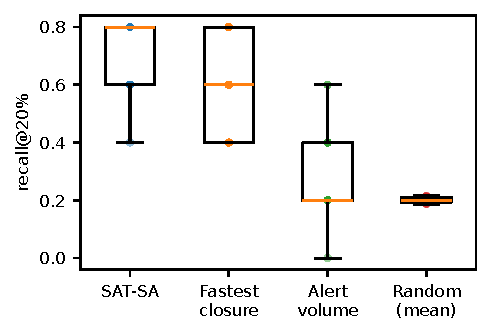
\includegraphics[width=\figscale{0.7}\linewidth]{figures/fig-prioritization.pdf}
\caption{Recall@20\% of generator-labelled pathological entities across generated
populations (PR01).}
\label{fig:prioritization}
\end{figure}

\subsection{Component ablation (RQ2)}

Removing one of the \V{A01-workers} workers at a time (Table~\ref{tab:ablation},
Figure~\ref{fig:ablation}), fast-closure and negative-space carried recall on the
catalog (recall \V{A01-fast-closure-recall} and \V{A01-negative-space-recall}
without them); removing evidence-completeness gave \V{A01-evidence-completeness-recall}.
Removing recurring-without-remediation or coverage-gap \emph{raised} precision
(\V{A01-recurring-without-remediation-precision}, \V{A01-coverage-gap-precision})
because those workers emitted only undeclared families here. On generated
populations (five seeds, exploratory), mean recall@20\% was
\V{A01-pop-full} with all workers, \V{A01-pop-fast-closure} without fast-closure
and \V{A01-pop-negative-space} without negative-space, while removing anomaly,
recurring-without-remediation, coverage-gap or workflow-reconstruction raised it to
\V{A01-pop-anomaly}: these workers add ranking noise on these populations. Several
workers had no measurable effect on these fixtures, which says only that the
fixtures do not exercise them.

% Generated by scripts/build_paper_assets.py from satsa-evidence-freeze-v2; do not edit.
% Sources: A01=EXP-A01-component-ablation (manifest 03632678da62b279)
\begin{table}[t]
\centering\small
\caption{One-worker ablation (A01): scenario micro metrics (5 scenarios) and mean population recall@20\% (5 seeds, exploratory). Workers with no change on either view are omitted.}
\label{tab:ablation}
\begin{adjustbox}{max width=\linewidth}
\begin{tabular}{lrrrr}
\toprule
Worker removed & Precision & Recall & F1 & Pop. R@20\% \\
\midrule
(full set) & 0.556 & 1.000 & 0.714 & 0.76 \\
-- fast-closure & 0.429 & 0.600 & 0.500 & 0.60 \\
-- recurring-without-remediation & 0.714 & 1.000 & 0.833 & 0.80 \\
-- negative-space & 0.500 & 0.600 & 0.545 & 0.64 \\
-- anomaly & 0.556 & 1.000 & 0.714 & 0.80 \\
-- peer-benchmark & 0.556 & 1.000 & 0.714 & 0.72 \\
-- coverage-gap & 0.625 & 1.000 & 0.769 & 0.80 \\
-- case-similarity & 0.556 & 1.000 & 0.714 & 0.72 \\
-- evidence-completeness & 0.500 & 0.800 & 0.615 & 0.76 \\
-- workflow-reconstruction & 0.556 & 1.000 & 0.714 & 0.80 \\
\bottomrule
\end{tabular}
\end{adjustbox}
\end{table}


\begin{figure}[t]
\centering
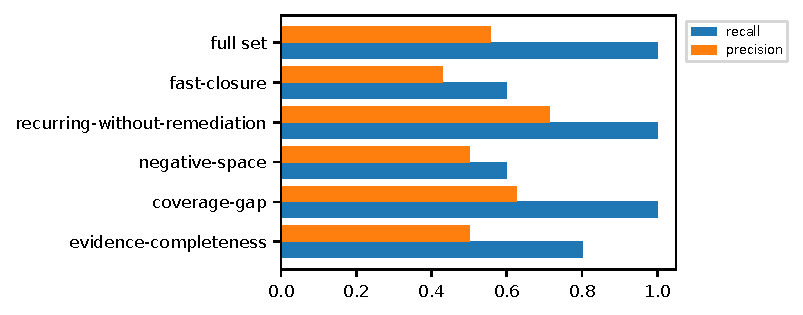
\includegraphics[width=\figscale{0.75}\linewidth]{figures/fig-ablation.pdf}
\caption{Catalog micro precision and recall with one worker removed; unchanged
removals omitted (A01).}
\label{fig:ablation}
\end{figure}

\subsection{Imperfect evidence (RQ4)}

Each of the perturbed conditions declared its family, affected records and
expected validation outcome before it ran, with one fresh tenant database per
condition. Hosted validation matched the declared contract in \V{R01b-match} of
\V{R01b-expect} conditions with an expectation; \V{R01b-na} were not applicable to
their fixture (Table~\ref{tab:robustness}). Exact and conflicting duplicates with
native identifiers, malformed timestamps, chronology violations and missing
columns were rejected (\V{R01b-malformation-invalid} malformation and
\V{R01b-duplication-invalid} duplication conditions).

Two behaviours matter for interpretation (Figure~\ref{fig:robustness}). First,
validation is all-or-nothing: independent record omission left dangling
references and rejected the whole submission in \V{R01b-ind10-rejected},
\V{R01b-ind25-rejected} and \V{R01b-ind50-rejected} of the seeded replicates at
10, 25 and 50\% omission, whereas referentially consistent omission was never
rejected and changed the emitted finding families in \V{R01b-cas10-changed},
\V{R01b-cas25-changed} and \V{R01b-cas50-changed} replicates. Second,
\textbf{stale and contradictory evidence is accepted silently}: all
\V{R01b-staleness-n} conditions with records outside the assessment period were
accepted with no warning and no change to findings or risk
(\V{R01b-stale-unchanged} unchanged), and contradictory dispositions or a closed
case with an open alert produced no finding. SAT-SA implements no period,
recency or cross-record consistency validation.

\widetable{tables/tab-robustness}

\begin{figure}[t]
\centering
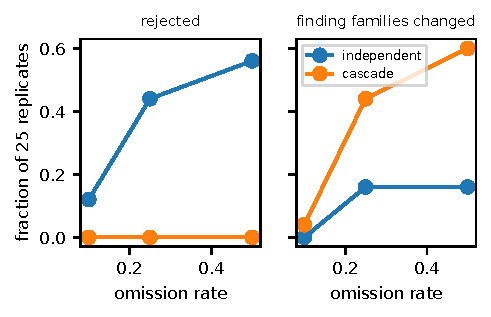
\includegraphics[width=\figscale{0.7}\linewidth]{figures/fig-robustness.pdf}
\caption{Record omission: independent omission is often rejected by all-or-nothing
validation; referentially consistent omission is accepted and changes findings more
often as the rate grows (R01b).}
\label{fig:robustness}
\end{figure}

\subsection{Peer-cohort sensitivity (RQ6)}

Over \V{P01-cells} engineered cells (Table~\ref{tab:peer},
Figure~\ref{fig:peer}), cohorts of two peers never produced a peer finding
(the rule requires three). With a tight cohort spread, \V{P01-tight-n3} of the
eight subject values were flagged from three peers upward---every value except the
one at the cohort median. With a wide spread only extreme slow subjects were
flagged at small cohorts (\V{P01-wide-n3} at three peers), and fast subjects were
flagged only from five peers upward as the MAD narrowed
(\V{P01-wide-n5} at five peers). The rule is therefore sensitive to cohort
dispersion and size, and small or heterogeneous cohorts will miss deviations.

% Generated by scripts/build_paper_assets.py from satsa-evidence-freeze-v2; do not edit.
% Sources: P01=EXP-P01-peer-sweep (manifest 7aa85508062b2b28)
\begin{table}[t]
\centering\small
\caption{Subjects flagged by the peer rule out of 8 subject values per cohort (P01).}
\label{tab:peer}
\begin{adjustbox}{max width=\linewidth}
\begin{tabular}{lrrrrrr}
\toprule
Spread & 2 peers & 3 & 4 & 5 & 6 & 8 \\
\midrule
tight & \V{P01-tight-n2} & \V{P01-tight-n3} & \V{P01-tight-n4} & \V{P01-tight-n5} & \V{P01-tight-n6} & \V{P01-tight-n8} \\
wide & \V{P01-wide-n2} & \V{P01-wide-n3} & \V{P01-wide-n4} & \V{P01-wide-n5} & \V{P01-wide-n6} & \V{P01-wide-n8} \\
\bottomrule
\end{tabular}
\end{adjustbox}
\end{table}


\begin{figure}[t]
\centering
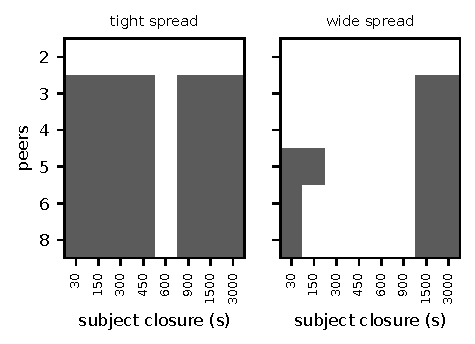
\includegraphics[width=\figscale{0.85}\linewidth]{figures/fig-peer.pdf}
\caption{Peer findings by cohort size, spread and subject closure value; dark cells
emitted a finding (P01).}
\label{fig:peer}
\end{figure}

\subsection{Orchestration cost and recovery (RQ7)}

On one machine with SQLite, \V{O01-pairs} paired trials per mode
(Table~\ref{tab:orchestration}, Figure~\ref{fig:orchestration}) gave median
processing times, excluding the human decision, of \V{O01-direct-median}\,s
(direct), \V{O01-graph-median}\,s (LangGraph) and \V{O01-unrev-median}\,s
(unreviewed benchmark mode). LangGraph minus direct was a median
\V{O01-diff-proc}\,s per workflow (\V{O01-diff-proc-rel} of the direct median; 95\%
bootstrap \V{O01-diff-proc-lo} to \V{O01-diff-proc-hi}\,s, graph slower in
\V{O01-diff-proc-greater} of \V{O01-pairs} pairs), with \V{O01-diff-db} more
database statements and \V{O01-checkpoints} checkpoints per run. Findings and risk
were identical across modes in every trial. Human review with TRUST-SAT
finalization added a median \V{O01-diff-review}\,s over unreviewed processing
(\V{O01-diff-review-lo} to \V{O01-diff-review-hi}\,s); finalization took a median
\V{O01-final-median}\,s (\V{O01-final-share} of reviewed processing), receipt
verification \V{O01-verify-median}\,s, and run and finding attestation
(\V{O01-attest-median}\,s) was the largest single cost. These are repeated
measurements on one machine; the intervals describe that variability only.

\widetable{tables/tab-orchestration}

\begin{figure}[t]
\centering
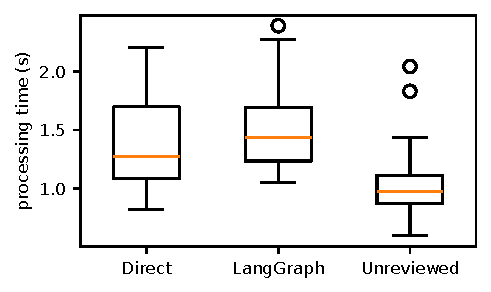
\includegraphics[width=\figscale{0.7}\linewidth]{figures/fig-orchestration.pdf}
\caption{Workflow processing time by execution mode on one machine with SQLite (O01).}
\label{fig:orchestration}
\end{figure}

Interruptions were injected at \V{O02-points} points in both modes with
\V{O02-trials} trials per cell (Table~\ref{tab:recovery}): transient failures and
simulated crashes (an exception bypassing the worker's handler followed by lease
expiry) during analysis, before recommendations, at a worker restart during review,
and during finalization. \textbf{In the evaluated interruption scenarios},
\V{O02-recovered} of \V{O02-runs} interrupted runs recovered to completion, and
\V{O02-identical} of them produced outputs identical to the uninterrupted
reference. Completed stages were repeated \V{O02-repeated} times; each run had
exactly one decision, one finalization and a verifying receipt. Real
process kills, network partitions and database failover were not exercised.

\widetable{tables/tab-recovery}
